% RescueSwarm research paper. IEEEtran conference format; pdflatex twice.
\documentclass[conference]{IEEEtran}
\IEEEoverridecommandlockouts

\usepackage{amsmath,amssymb}
\usepackage{graphicx}
\usepackage{booktabs}
\usepackage{array}
\usepackage{url}
\usepackage{tikz}
\usetikzlibrary{shapes.geometric,arrows.meta,positioning,fit,calc,backgrounds}
\usepackage[hidelinks]{hyperref}

\graphicspath{{../proposal/figures/}{../../ground-station/}}

\tikzset{
  blk/.style   ={draw, rounded corners=2pt, align=center, font=\scriptsize,
                 minimum height=6mm, inner sep=3pt},
  seg/.style   ={draw, dashed, rounded corners=4pt, inner sep=5pt},
  dec/.style   ={draw, diamond, aspect=2.2, align=center, font=\scriptsize,
                 inner sep=1pt},
  flow/.style  ={-{Stealth[length=2mm]}, thick},
  dflow/.style ={-{Stealth[length=2mm]}, dashed},
  lbl/.style   ={font=\scriptsize\itshape, inner sep=1pt},
}

\begin{document}

\title{Design and Simulation-Based Evaluation of a\\
Three-Aircraft Autonomous System for Post-Flood\\
Search, Geolocation and Relief Delivery}

\author{
\IEEEauthorblockN{Swastik Kumar}
\IEEEauthorblockA{\textit{Department of Electronics \& Communication Engineering} \\
\textit{Thapar Institute of Engineering \& Technology}\\
Patiala, Punjab, India \\
skumar6\_be24@thapar.edu}
}

\maketitle

\begin{abstract}
Finding survivors is usually the slowest step of a flood rescue. We describe
RescueSwarm, a system of three multirotor aircraft that search an assigned area
under one operator, detect people from 40\,m, report each one as a map
coordinate and drop a 200\,g relief kit to them, all without a mobile network.
The paper covers the design and its evaluation by analysis and
software-in-the-loop simulation; no aircraft has flown yet. Four results stand
out. First, a Monte Carlo geolocation budget shows that about 0.88\,m of
coordinate error comes from sources no receiver can remove, so any receiver with
horizontal error below 2.75\,m meets a 5\,m delivery requirement at 95\,\%
confidence; RTK gives 1.53\,m and standalone NavIC, at 8.79\,m, does not. Second,
a person in water at 40\,m covers 1\,498\,px$^2$ only if the 12\,MP frame is
tiled at full resolution, and either halving the resolution or flying at 60\,m
pushes the target into the small-object range where detectors are weakest.
Third, a single 802.11 mesh would have left 8.7\,dB of margin at the 600\,m
geofence, so we split traffic over three radios with at least 29.7\,dB each,
and found that LoRa framing overhead, not bit rate, limits the coordination
channel. Fourth, in simulation with three ArduCopter autopilots, staggering
take-off in the mission file raised the closest approach at launch from 1.31\,m
to 26.96\,m.
\end{abstract}

\begin{IEEEkeywords}
unmanned aerial systems, multi-robot coordination, search and rescue,
geolocation error, small object detection, link budget, disaster response
\end{IEEEkeywords}

%=============================================================================
\section{Introduction}
%=============================================================================

India recorded 5.4 million internal displacements from disasters in 2024, the
most in twelve years, and 2.4 million of them came from one monsoon flood season
in Assam~\cite{idmc2025grid}. In a flood, boat crews and ground teams reach
people reliably once they know where to go. The hard part is knowing where to
go. Boats search slowly and cover rooftops and debris poorly, and the few
helicopters available are mostly flying evacuations.

Small multirotors could take over much of that search, but one aircraft carrying
a useful payload for fifteen minutes covers little ground, and a team that needs
one pilot per aircraft does not scale. We therefore set out to design a small
fleet that one person can supervise. Three aircraft divide an area, sweep it,
detect people on board, agree among themselves who serves each survivor, and
drop a kit. The design target was a first-response team in the field, so the
system carries its own positioning base and radios and needs no internet or
mobile service.

Building such a system mostly means trading one requirement against another,
and the trades are where we think the useful findings are. This paper reports
them. Its contributions are:
\begin{enumerate}
  \item a geolocation error budget, checked by Monte Carlo simulation, that
        gives the receiver accuracy needed for a 5\,m delivery requirement and
        shows how little of the error the receiver controls;
  \item an analysis of detection geometry for a person in water, showing why
        survey altitude and tiling resolution have to be chosen together;
  \item a link and channel-occupancy analysis that led us from one mesh network
        to three single-purpose radios;
  \item a battery analysis covering pack selection at the aircraft's own mass
        and the dynamic voltage sag seen by the low-battery failsafe; and
  \item software-in-the-loop results for launch, sweep and recovery with three
        autopilots running together.
\end{enumerate}

None of the aircraft has flown. Every result here is either computed from a
model or measured in simulation, and we say which in each case.

%=============================================================================
\section{Related Work}
%=============================================================================

\textit{Coverage and allocation.} DARP divides an area into equal, connected
regions, one per robot~\cite{kapoutsis2017darp}, and boustrophedon decomposition
remains the usual way to sweep a rectangular sensor footprint across a
region~\cite{choset2000coverage}. For assigning tasks among agents, the
consensus-based bundle algorithm is the common decentralised
choice~\cite{choi2009cbba}. We use a fixed equal-area split with boustrophedon
coverage inside each strip, and a greedy claim-and-lock rule for survivors. With
three aircraft, each linked to one ground station, the guarantees that CBBA
offers add little, and a plan that is the same every time the inputs are the
same is much easier to test.

\textit{Detecting people from the air.} People seen from survey altitude are
tiny. COCO counts anything under 32$^2$\,px$^2$ as a small
object~\cite{lin2014coco}, and TinyPerson adds finer bands below that because
aerial images of people are often smaller still~\cite{yu2020tinyperson}.
Running the detector on overlapping crops of the full-resolution frame, as in
SAHI, recovers much of the recall lost on small objects~\cite{akyon2022sahi}.
Relevant datasets include SARD for land search~\cite{sambolek2021sard},
VisDrone for urban scenes~\cite{zhu2021visdrone} and SeaDronesSee, which labels
people in open water~\cite{varga2022seadronessee}. The last is closest to a
flood, with a low-contrast background and targets that show only head and
shoulders, but none of them covers flooded Indian terrain.

\textit{Airdrop and positioning.} Mathisen \emph{et al.} reported autonomous
ballistic airdrop from a small fixed-wing aircraft with a mean error of
5.5\,m, and found that aircraft velocity and wind at release dominate the
error~\cite{mathisen2020airdrop}. A multirotor can almost stop before releasing,
which removes the largest of those terms. For positioning without a network,
real-time kinematic (RTK) correction from a local base station is the standard
way to reach sub-metre relative accuracy~\cite{takasu2009rtklib}.

%=============================================================================
\section{System Design}
%=============================================================================

\subsection{Architecture}

Fig.~\ref{fig:arch} shows the three parts of the system. Each aircraft is an
18\,in quadrotor with a Holybro Kakute~H7 autopilot running
ArduPilot~\cite{ardupilot}, a u-blox ZED-F9P dual-band RTK
receiver~\cite{ubloxzedf9p}, a downward-facing 12.3\,MP camera, a Raspberry Pi~5
companion computer with a 26\,TOPS neural accelerator, a four-station kit
magazine with mechanical locks, and three radios. The ground segment is a single
station and one operator. A second ZED-F9P on a tripod acts as the RTK base and
sends corrections over its own 865\,MHz radio. The companion forwards them to
the autopilot, which passes them to the receiver.

\begin{figure}[t]
\centering
\resizebox{\columnwidth}{!}{%
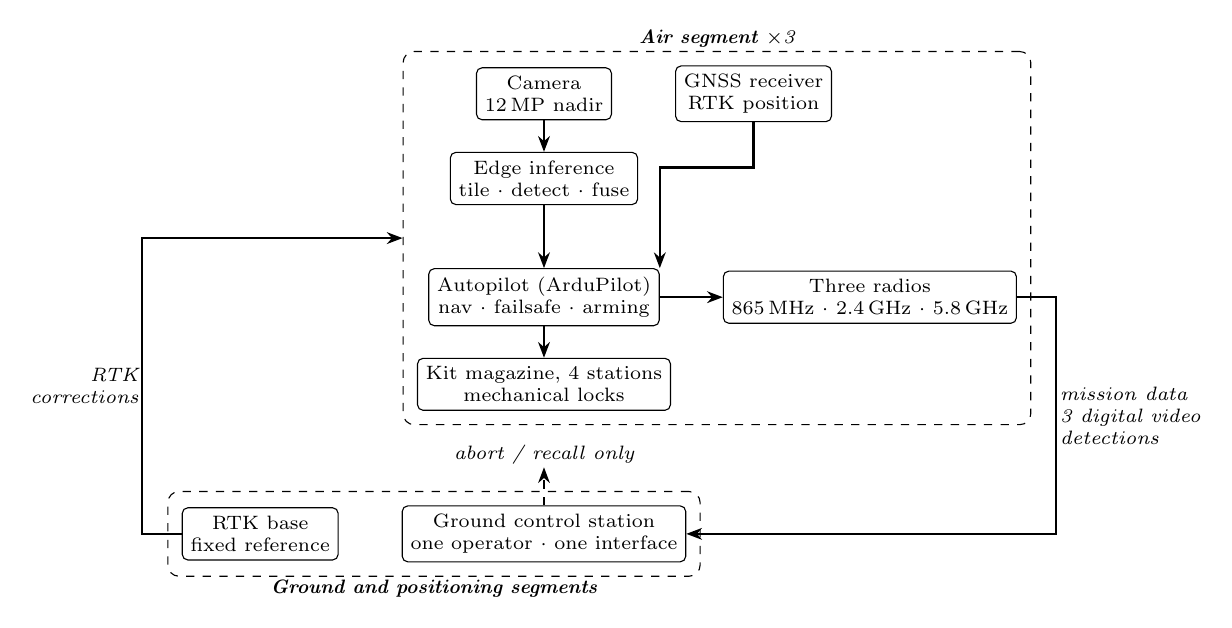
\begin{tikzpicture}[node distance=4mm]
\node[blk] (cam)  {Camera\\12\,MP nadir};
\node[blk, right=8mm of cam] (gnss) {GNSS receiver\\RTK position};
\node[blk, below=4mm of cam] (inf) {Edge inference\\tile $\cdot$ detect $\cdot$ fuse};
\node[blk, below=8mm of inf] (fc) {Autopilot (ArduPilot)\\nav $\cdot$ failsafe $\cdot$ arming};
\node[blk, right=8mm of fc] (rad) {Three radios\\865\,MHz $\cdot$ 2.4\,GHz $\cdot$ 5.8\,GHz};
\node[blk, below=4mm of fc] (mag) {Kit magazine, 4 stations\\mechanical locks};
\draw[flow] (cam) -- (inf);
\draw[flow] (inf) -- (fc);
\draw[flow] (gnss) -- (gnss|-inf.north) -- ++(0,-2mm) -| (fc.north east);
\draw[flow] (fc) -- (mag);
\draw[flow] (fc) -- (rad);
\begin{scope}[on background layer]
\node[seg, fit=(cam)(gnss)(inf)(fc)(rad)(mag),
      label={[lbl]above:\textbf{Air segment} $\times$3}] (air) {};
\end{scope}
\node[blk, below=12mm of mag] (gcs) {Ground control station\\one operator $\cdot$ one interface};
\node[blk, left=8mm of gcs] (rtk) {RTK base\\fixed reference};
\begin{scope}[on background layer]
\node[seg, fit=(gcs)(rtk),
      label={[lbl]below:\textbf{Ground and positioning segments}}] (gnd) {};
\end{scope}
\draw[flow] (rad.east) -- ++(5mm,0) |- (gcs.east)
      node[lbl, pos=0.25, right, align=left]
      {mission data\\3 digital video\\detections};
\draw[dflow] (gcs.north) -- (gcs.north|-gnd.north) -- ++(0,3mm)
      node[lbl, above, align=center] {abort / recall only};
\draw[flow] (rtk.west) -- ++(-5mm,0) |- (air.west)
      node[lbl, pos=0.25, left, align=right] {RTK\\corrections};
\end{tikzpicture}}
\caption{System architecture. Detection runs on board, so the downlink serves
the operator rather than the detector. The only commands the ground station can
send are abort and recall.}
\label{fig:arch}
\end{figure}

The ground station cannot retask an aircraft, move a waypoint or order a drop.
We left those commands out of the software entirely rather than disabling them,
so they cannot be switched on by mistake. Safety control comes from a separate
2.4\,GHz ExpressLRS link wired straight to the autopilot, so the safety pilot
keeps control if the companion computer hangs.

\subsection{Mission and coordination}

During setup the operator draws the search area, which is split into three
strips of equal area, one per aircraft. Each strip is swept back and forth at
40\,m and 8\,m/s. Before upload, the planner tries all four combinations of
starting side and sweep direction and keeps the one that ends nearest the pad,
because the return leg is flown on the emptiest battery. Take-off delays of 0,
15 and 30\,s and transit altitudes of 20, 25 and 30\,m are written into the
mission files, so separation does not depend on the operator's timing.

When an aircraft confirms a survivor it broadcasts a claim. If two aircraft
claim the same survivor, the one with the lower identifier keeps it. Abnormal
conditions all end the same way: loss of link for more than 60\,s, low battery
and an operator abort each lead to return-to-launch. Below a second, lower
battery threshold the aircraft lands where it is.

\subsection{Onboard processing}

The autopilot flies the search as an ordinary \textsc{auto} mission and would
complete it with the companion computer switched off (Fig.~\ref{fig:pipeline}).
The companion detects, locates and claims survivors, and takes control only for
a delivery: a short \textsc{guided} manoeuvre to descend, stop and release,
after which the \textsc{auto} mission resumes. A crash of the companion
therefore costs detections, not the aircraft.

\begin{figure}[t]
\centering
\resizebox{0.92\columnwidth}{!}{%
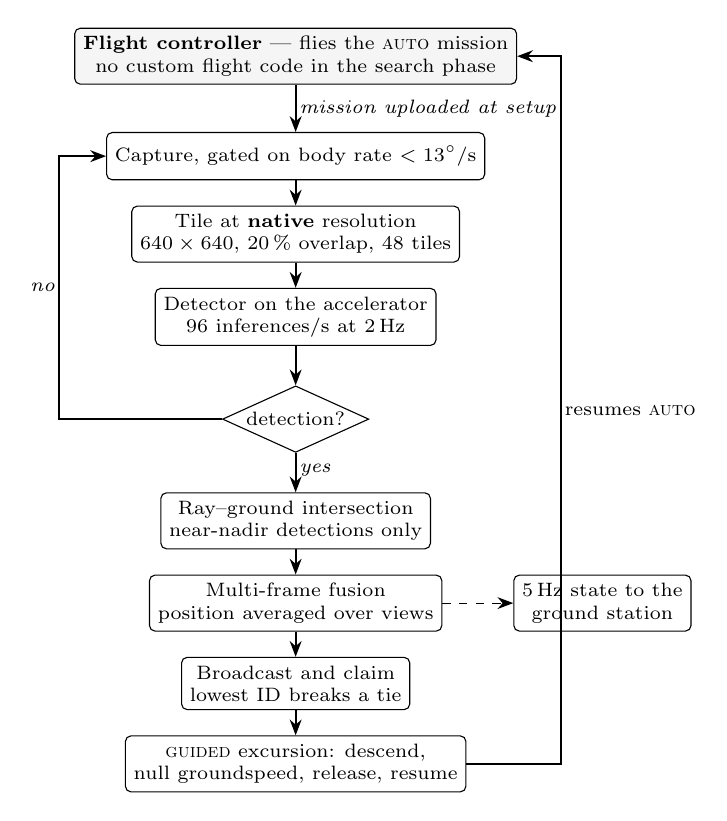
\begin{tikzpicture}[node distance=3.2mm]
\node[blk, fill=black!4] (fc) {\textbf{Flight controller} --- flies the
\textsc{auto} mission\\no custom flight code in the search phase};
\node[blk, below=6mm of fc] (cap) {Capture, gated on body rate
$<13^\circ$/s};
\node[blk, below=of cap] (tile) {Tile at \textbf{native} resolution\\$640\times640$,
20\,\% overlap, 48 tiles};
\node[blk, below=of tile] (det) {Detector on the accelerator\\96 inferences/s
at 2\,Hz};
\node[dec, below=5mm of det] (hit) {detection?};
\node[blk, below=5mm of hit] (ray) {Ray--ground intersection\\near-nadir
detections only};
\node[blk, below=of ray] (fuse) {Multi-frame fusion\\position averaged over views};
\node[blk, below=of fuse] (claim) {Broadcast and claim\\lowest ID breaks a
tie};
\node[blk, below=of claim] (del) {\textsc{guided} excursion: descend,\\null
groundspeed, release, resume};
\node[blk, right=9mm of fuse, align=center] (pub) {5\,Hz state to the\\ground
station};
\draw[flow] (fc) -- node[lbl, right] {mission uploaded at setup} (cap);
\draw[flow] (cap) -- (tile);
\draw[flow] (tile) -- (det);
\draw[flow] (det) -- (hit);
\draw[flow] (hit) -- node[lbl, right, pos=0.45] {yes} (ray);
\draw[flow] (ray) -- (fuse);
\draw[flow] (fuse) -- (claim);
\draw[flow] (claim) -- (del);
\coordinate (fb) at ([xshift=-6mm]cap.west);
\draw[flow] (hit.west) -- (fb |- hit) -- node[lbl, left, pos=0.5] {no}
  (fb) -- (cap.west);
\draw[dflow] (fuse.east) -- (pub.west);
\draw[flow] (del.east) -- ++(12mm,0) |- node[lbl, font=\scriptsize, pos=0.25, right]
  {resumes \textsc{auto}} (fc.east);
\end{tikzpicture}}
\caption{Onboard processing. Detection runs alongside the sweep and never holds
it up. Frames are not captured in turns, where motion blur is worst: one pixel
spans 13.63\,mdeg, so at a $1/1000$\,s exposure a rotation of
$13.6^\circ$/s blurs by one pixel, and the gate is set just below that.}
\label{fig:pipeline}
\end{figure}

%=============================================================================
\section{Aircraft Sizing and Energy}
\label{sec:sizing}
%=============================================================================

\subsection{Power and mass}

We sized the aircraft with momentum theory~\cite{leishman2006helicopter}, using
cautious constants: air density of 1.150\,kg/m$^3$ for a hot day at 300\,m, a
figure of merit of 0.60, motor and controller efficiencies of 0.82 and 0.95,
and 55\,W of avionics. Four 18\,in rotors give 0.657\,m$^2$ of disk area. Hover
shaft power is
\begin{equation}
P_{\text{shaft}} = \frac{T^{3/2}}{\mathrm{FM}\sqrt{2\rho A}} = 668~\text{W}
\end{equation}
at a take-off mass of 6.36\,kg, or 913\,W of electrical power once drivetrain
losses and avionics are added. That is 42.2\,A at 21.6\,V. At the design
thrust-to-weight ratio of 2.0 the electrical power rises to 2\,481\,W and the
current to 114.8\,A. Hover takes 1.59\,kgf per motor, half the 3.18\,kgf each
motor must produce at full thrust.

The motor we selected is rated for 26.5\,A continuous. It draws 10.6\,A in
hover and 28.7\,A at full thrust, 108\,\% of its rating. We accept that only
because full thrust is a gust reserve lasting seconds, and it is the tightest
margin in the propulsion system. Pack mass, take-off mass and mission energy
depend on one another, so the model iterates until they settle. Structure and
battery make up 46\,\% of the take-off mass, the four kits 12.6\,\%. The fleet
of three weighs 19.08\,kg, inside the 25\,kg limit of the Indian drone
rules~\cite{dronerules2021}.

\subsection{Reserve and pack selection}

The battery is sized by its reserve, not by the mission. The pack has to supply
the 103.4\,Wh mission, a complete second sweep (30.9\,Wh) for the case where
the first finds nothing, and four minutes of hover (60.8\,Wh) while three
aircraft queue to land. That is 195.2\,Wh usable, or at least 244\,Wh rated if
we never discharge below 20\,\%.

The model was first solved for an 18-cell 6S3P Li-ion pack. We then compared
ready-made LiPo packs, each evaluated at its own mass, since a heavier pack
needs more hover power (Table~\ref{tab:packs}). A 12 or 13\,Ah pack fails both
the endurance and the landing-queue requirement, about 14\,Ah is the smallest
that passes, and we chose a 6S 16\,Ah high-voltage LiPo, the smallest suitable
size sold in India. It also removes the need to spot-weld eighteen cells, the
most hazardous step of the original build. The cost is thrust-to-weight: at
6.8--7.1\,kg the motors give 1.8--1.9 unless each produces at least 3.55\,kgf.

\begin{table}[t]
\caption{Flight pack candidates, each evaluated at its own mass}
\label{tab:packs}
\centering
\footnotesize
\setlength{\tabcolsep}{3pt}
\begin{tabular}{@{}lrrrrr@{}}
\toprule
\textbf{Pack} & \textbf{kg} & \textbf{Wh} & \textbf{T/W} & \textbf{Endur.} & \textbf{Queue, Wh} \\
\midrule
Li-ion 6S3P       & 1.45 & 292 & 2.00 & 2.02 & $+$1.1 \\
LiPo 12\,Ah       & 1.42 & 266 & 2.01 & 1.85$^\ast$ & $-$3.7$^\ast$ \\
LiPo 13\,Ah       & 1.52 & 289 & 1.98 & 1.96$^\ast$ & $-$0.5$^\ast$ \\
LiPo 14\,Ah       & 1.64 & 311 & 1.94 & 2.06 & $+$2.5 \\
\textbf{LiPo 16\,Ah HV} & \textbf{1.88--2.21} & \textbf{365} & \textbf{1.8--1.9} & \textbf{2.1--2.3} & \textbf{$+$5 to $+$9} \\
\bottomrule
\multicolumn{6}{@{}p{8.4cm}@{}}{\footnotesize Endurance is hover time divided
by mission time and must be at least 2.0. Queue is what remains of the 20\,\%
reserve after the third aircraft waits 120\,s. $^\ast$\,Fails. The maker does
not publish the 16\,Ah pack's mass, so it is bracketed at 165--194\,Wh/kg.}
\end{tabular}
\end{table}

\subsection{Voltage sag and the failsafe}

A static resistance figure is enough to size a pack but not to set a failsafe,
because it says nothing about when in the flight the voltage is lowest or how
long a dip lasts. We simulated the chosen pack with a second-order Thevenin
cell model,
\begin{equation}
v = \mathrm{OCV}(z) - iR_0 - v_1 - v_2,\qquad
\dot v_k = -\frac{v_k}{R_kC_k} + \frac{i}{C_k},
\end{equation}
with time constants of about 5\,s and 90\,s and a constant-power load, so that
current rises as voltage falls. The load is the mission profile scaled to the
heaviest likely mass of 7.1\,kg, with two two-second full-thrust gust
recoveries added at 300\,s and 430\,s (Fig.~\ref{fig:sag}).

\begin{figure*}[t]
\centering
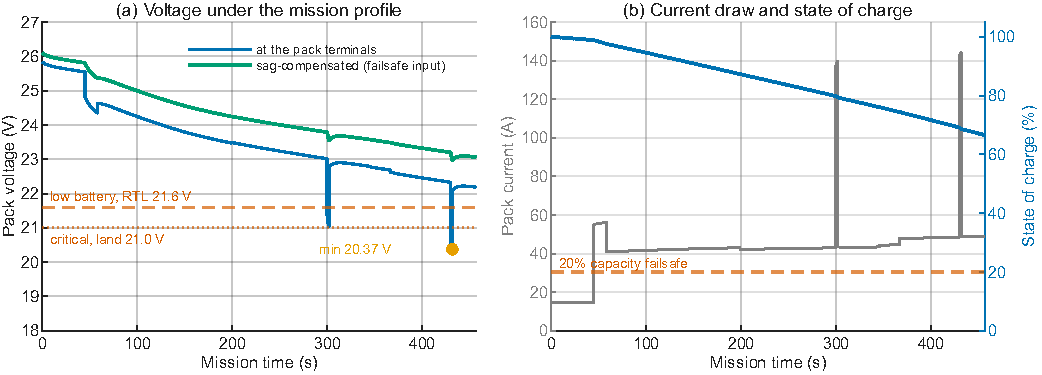
\includegraphics[width=\textwidth]{fig-sag.pdf}
\caption{Simulated voltage of the 6S 16\,Ah LiPo over the mission at 7.1\,kg,
with two full-thrust gust recoveries. (a) Terminal voltage dips to 20.37\,V,
below the 21.6\,V low-battery threshold, but the sag-compensated voltage the
failsafe compares never falls below 22.97\,V. (b) Current peaks at 144\,A and
the aircraft lands at 66\,\% charge. Cell resistances are typical values, not
measurements.}
\label{fig:sag}
\end{figure*}

The terminal voltage falls to 20.37\,V during the late gust, below the 21.6\,V
low-battery threshold, at a point where the pack is still two-thirds full. A
failsafe that compared raw voltage would send a healthy aircraft home. ArduPilot
avoids this in two ways. It estimates the pack's internal resistance as it flies
and compares a voltage corrected for the present current, and it acts only
after the voltage has stayed low for 10\,s. In our run the corrected voltage
stays at or above 22.97\,V. The low-battery action is in any case set on
consumed capacity, at 20\,\% remaining, with voltage as a backstop. The
simulation also gives a peak current of 144\,A, close to the 150\,A rating of
the fuse and connectors, which makes the fuse the tightest electrical margin on
the aircraft.

%=============================================================================
\section{Geolocation Error}
\label{sec:geotag}
%=============================================================================

\subsection{Error budget}

A survivor coordinate comes from projecting a pixel through the camera model
onto a ground plane, using the aircraft's position and attitude. We modelled the
total error as the root sum of squares (RSS) of independent terms and checked
it by Monte Carlo simulation with 200\,000 samples per case, treating each term
as a two-axis Gaussian. The simulation agrees with the analytic circular
Gaussian result, CEP50\,$=0.8326\times$RSS, to within one per cent.

With RTK the receiver contributes about 1\,cm, which is negligible. Two terms
that no receiver can reduce dominate: unmodelled error, set at 0.70\,m, and the
size and centring of the target, 0.50\,m (Fig.~\ref{fig:geobudget}). Together
they account for 95\,\% of the variance. The remaining terms are boresight
residual (0.16\,m), the GNSS-to-camera lever arm (0.10\,m), attitude (0.07\,m)
and pixel centroiding (0.02\,m). Excluding the receiver, the budget adds to
0.88\,m.

\begin{figure*}[t]
\centering
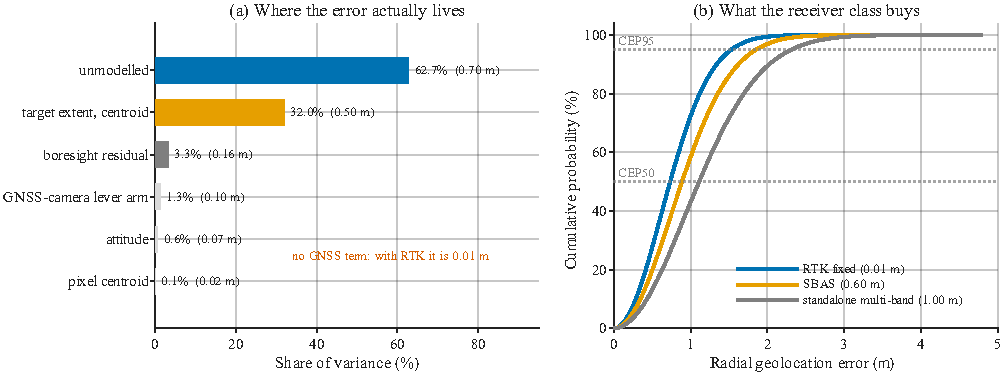
\includegraphics[width=\textwidth]{fig-geobudget.pdf}
\caption{(a) Sources of geolocation error with RTK. Unmodelled error and target
centring account for 95\,\% of the variance. (b) Radial error by receiver class,
200\,000 Monte Carlo samples. RTK and SBAS differ by only 0.16\,m in CEP50.}
\label{fig:geobudget}
\end{figure*}

Combining views of the same target helps, but not by $1/\sqrt{n}$. At 40\,m the
footprint is 31.4\,m long, so at 8\,m/s a target stays in view for 3.9\,s and
is seen about eight times at a 2\,Hz detection rate. Averaging reduces the
random terms but not boresight error or target size, so the curve flattens by
about five views. A single-frame fix without RTK gives 3.09\,m RSS, and RTK with
a single frame about 1.3\,m. RTK with multi-frame fusion and a calibrated ground
plane gives 0.91\,m, or 0.94\,m when attitude comes from the compass instead of
a second receiver.

\subsection{Required receiver accuracy}

Adding a receiver error $\sigma_g$ in quadrature to the 0.88\,m floor and
converting to the 95\,\% radius gives the requirement directly:
\begin{equation}
\mathrm{CEP95} = 1.7308\sqrt{\sigma_{\mathrm{rest}}^{2} + \sigma_g^{2}}
\;\le\; 5\,\text{m}
\;\Longrightarrow\;
\sigma_g \le 2.75\,\text{m}.
\label{eq:gnssbreak}
\end{equation}
Table~\ref{tab:receivers} and Fig.~\ref{fig:receivers} apply this to five
classes of receiver. RTK, SBAS and autonomous multi-band receivers all clear the
requirement, and GPS L1 alone is marginal at 4.59\,m. NavIC at its published
standalone accuracy gives 8.79\,m and fails. NavIC is still useful as an extra
constellation for satellite geometry, but it cannot replace the correction.

\begin{table}[t]
\caption{Receiver classes against a 5\,m delivery requirement}
\label{tab:receivers}
\centering
\small
\begin{tabular}{@{}lrrrl@{}}
\toprule
\textbf{Class} & $\boldsymbol{\sigma_g}$ & \textbf{CEP50} & \textbf{CEP95} & \\
\midrule
RTK fixed             & 0.01\,m & 0.74\,m & \textbf{1.53\,m} & clears \\
SBAS / GAGAN          & 0.60\,m & 0.89\,m & \textbf{1.85\,m} & clears \\
Multi-band autonomous & 1.00\,m & 1.11\,m & \textbf{2.31\,m} & clears \\
GPS L1 only           & 2.50\,m & 2.21\,m & \textbf{4.59\,m} & marginal \\
NavIC SPS             & 5.00\,m & 4.23\,m & \textbf{8.79\,m} & \emph{fails} \\
\bottomrule
\end{tabular}
\end{table}

\begin{figure*}[t]
\centering
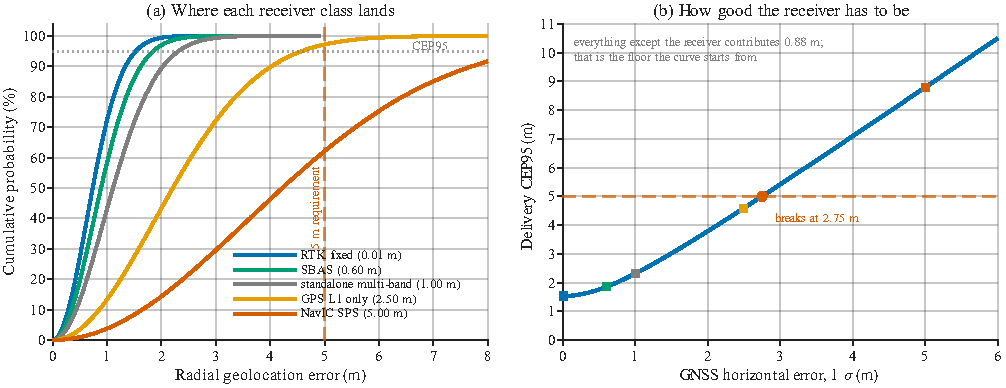
\includegraphics[width=\textwidth]{fig-receivers.pdf}
\caption{(a) Radial error distributions for five receiver classes, 200\,000
samples each. (b) Delivery CEP95 against the receiver's horizontal error, with
the 5\,m requirement and the 2.75\,m limit of (\ref{eq:gnssbreak}). The curve
starts at 0.88\,m because that part of the budget is independent of the
receiver.}
\label{fig:receivers}
\end{figure*}

The SBAS value of 0.60\,m is optimistic, and field results are nearer
1.0--1.5\,m. That still gives 2.31--3.01\,m, so the conclusion holds. Since the
mission requirement does not need RTK, we keep it for a different reason.
Measuring detection recall and delivery error in field trials requires the
geometry between targets, aircraft and pad to be known to centimetres, and that
is what RTK provides. A ZED-F9P rover with antenna and compass now costs about
as much as the receiver and separate compass it replaces, so every aircraft
carries one.

The base takes its position from its first three-dimensional fix rather than
from a survey-in. This saves many minutes of setup but shifts every reported
coordinate by the same absolute error, around a metre. The relative accuracy
between aircraft is unaffected. A rescue crew navigating with its own
metre-class receiver will barely notice the shift, and twenty minutes of
survey-in would come straight out of the flying time.

%=============================================================================
\section{Detection Geometry}
\label{sec:perception}
%=============================================================================

The camera has $4056\times3040$ pixels at 1.55\,\textmu m behind a 6\,mm lens,
giving fields of view of $55.3^\circ\times42.9^\circ$ and a ground sample
distance of 1.03\,cm/px at 40\,m. We design for the hardest target, a person in
water with only head and shoulders showing, about 0.4\,m across. An adult lying
on a roof is about four times larger in the image.

The important quantity is the size class the target falls into, because
detector accuracy is reported by size class and drops sharply for small objects.
Table~\ref{tab:target} gives the person-in-water target for four combinations of
altitude and tiling. Only one of them, 40\,m with the full-resolution frame cut
into 48 overlapping $640\times640$ tiles, keeps the target above the COCO
small-object threshold (Fig.~\ref{fig:detect}). Flying higher or halving the
resolution on its own is enough to push it below. At 50\,m the target is already
down to 959\,px$^2$.

\begin{table}[t]
\caption{Person-in-water target size by altitude and tiling}
\label{tab:target}
\centering
\small
\begin{tabular}{@{}llrrl@{}}
\toprule
\textbf{Altitude} & \textbf{Tiling} & \textbf{px} & \textbf{px$^2$} & \textbf{COCO class} \\
\midrule
\textbf{40\,m} & \textbf{native} & \textbf{39} & \textbf{1\,498} & medium \\
60\,m & native & 26 & 666 & small \\
40\,m & $2\times$ downsample & 19 & 375 & small \\
60\,m & $2\times$ downsample & 13 & 166 & small \\
\bottomrule
\end{tabular}
\end{table}

\begin{figure*}[t]
\centering
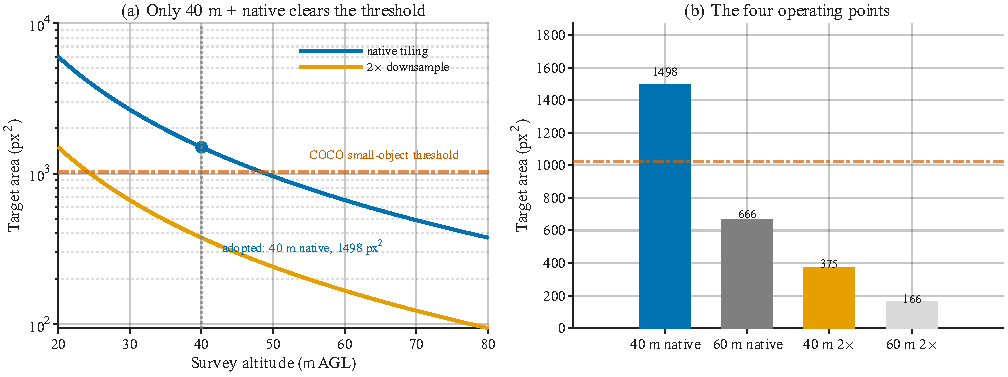
\includegraphics[width=\textwidth]{fig-detect.pdf}
\caption{Target area against survey altitude for a person in water. (a) Only
40\,m with full-resolution tiling stays above the COCO small-object threshold;
halving the resolution puts the target below it at every altitude. (b) The four
candidate settings.}
\label{fig:detect}
\end{figure*}

Full-resolution tiling has a cost in computing. At 2\,Hz, 48 tiles per frame
means 96 detector runs per second, against 130--160 per second published for
this accelerator with the same model and input size. The 2\,Hz rate gives 7.9
views per target, short of the twelve we would like for confirmation, and
reaching twelve would need 3.06\,Hz and 147 runs per second, at or beyond the
accelerator's limit. A cheap first stage that rejects tiles of open water would
free that capacity, which makes the case for a two-stage detector one of
throughput rather than accuracy. We have not yet benchmarked our own model and
tiling on this hardware, so these throughput numbers are the least certain in
the paper.

The rest of the optics is unproblematic. The hyperfocal distance is 4.15\,m, so
a fixed-focus lens is sharp at every altitude flown. Keeping motion blur under a
pixel at 8\,m/s needs an exposure of 1/774\,s or shorter, and we require
1/1000\,s. The rolling-shutter readout of 25\,ms skews the frame by 0.20\,m,
which does not affect detection but must be corrected in geolocation.

%=============================================================================
\section{Radio Links}
\label{sec:links}
%=============================================================================

\subsection{From one mesh to three radios}

Our first design carried video, telemetry and coordination on one 5.8\,GHz
802.11 mesh. Applying the link margin
\begin{equation}
M = P_{\mathrm{tx}} + G_{\mathrm{tx}} + G_{\mathrm{rx}}
    - \mathrm{FSPL}(f,d) - S_{\mathrm{rx}}
\label{eq:margin}
\end{equation}
at the 600\,m geofence, with 20\,dBm into 5\,dBi antennas and an MCS0
sensitivity of $-82$\,dBm, left 8.7\,dB. The link carrying the most traffic
would have been the weakest. Relaying through another aircraft does not help
much, because the things that break the direct path, such as a banked airframe,
a person in the way or rain, tend to affect both hops.

We replaced the mesh with three radios, each carrying one kind of traffic
(Table~\ref{tab:links}). Digital video runs on wfb-ng~\cite{wfbng} at
5.8\,GHz, one channel per aircraft, with a 14\,dBi panel antenna at the ground
for each. Command and abort run on ExpressLRS at 2.4\,GHz, which also carries
MAVLink telemetry~\cite{elrsmavlink}. Mission data and coordination run on an
SX1262 at 865\,MHz, which is licence-free in India. Every link now has at least
29.7\,dB of margin at the geofence (Fig.~\ref{fig:links}). The cost is that one
aircraft can no longer relay for another, a case the link-loss failsafe already
handles.

\begin{table}[t]
\caption{Radio links at the 600\,m geofence}
\label{tab:links}
\centering
\small
\setlength{\tabcolsep}{4pt}
\begin{tabular}{@{}lrrrrr@{}}
\toprule
 & $P_{\mathrm{tx}}$ & $\Sigma G$ & $S_{\mathrm{rx}}$ & FSPL & $M$ \\
\textbf{Link} & (dBm) & (dBi) & (dBm) & (dB) & (dB) \\
\midrule
Digital video, 5.8\,GHz & 27.0 & 20 & $-86$ & 103.3 & \textbf{29.7} \\
ExpressLRS, 2.4\,GHz & 20.0 & 4 & $-108$ & 95.6 & \textbf{36.4} \\
LoRa, 865\,MHz SF7 & 14.0 & 4 & $-123$ & 86.7 & \textbf{54.3} \\
\midrule
\emph{802.11 mesh, 5.8\,GHz} & 20.0 & 10 & $-82$ & 103.3 & \emph{8.7} \\
\bottomrule
\end{tabular}
\end{table}

\begin{figure*}[t]
\centering
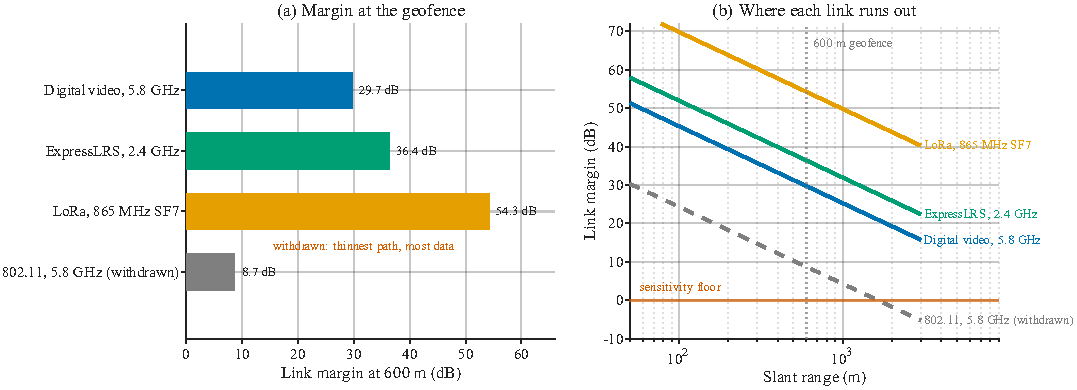
\includegraphics[width=\textwidth]{fig-links.pdf}
\caption{(a) Link margin at the 600\,m geofence, with the abandoned 802.11 mesh
for comparison. (b) Margin against distance. The mesh reaches its sensitivity
limit at 1.64\,km; the video link would reach 18.4\,km.}
\label{fig:links}
\end{figure*}

\subsection{Sizing the coordination channel}

Splitting the links had a consequence the margin table hides. The mesh offered
about 235\,kbps of non-video capacity per aircraft. LoRa at SF7 on a 125\,kHz
channel offers 5\,469\,bps for the whole fleet. What limits the channel,
though, is airtime rather than bit rate, because for short packets the preamble
and header dominate. A 36-byte frame at SF7 takes 77.1\,ms on air, where its
payload alone would take 52.7\,ms.

Sending state, coordination and detections as three separate messages per
aircraft per second used 28.4\,\% of the channel, above the 25\,\% we allow for
retries. Packing them into one 36-byte frame brought this to 25.3\,\%, with
nothing to spare. The 54.3\,dB margin pointed to the answer: the spreading
factor was buying range we did not need. The same SX1262 can run GFSK at
50\,kbps with a sensitivity of $-104$\,dBm. That gives up 19\,dB of margin,
leaving 35.3\,dB, and cuts each frame to 7.8\,ms and channel use to 2.3\,\%
(Table~\ref{tab:coord}). We use GFSK normally and fall back to LoRa SF7 at a
lower message rate when the link weakens.

\begin{table}[t]
\caption{Coordination channel, three aircraft, one 36\,B frame each at 1\,Hz}
\label{tab:coord}
\centering
\small
\begin{tabular}{@{}lrrrr@{}}
\toprule
\textbf{Mode} & \textbf{Rate} & \textbf{Frame} & \textbf{Occupancy} & \textbf{Margin} \\
\midrule
GFSK 50\,kbps      & 50\,kbps & 7.8\,ms & \textbf{2.3\,\%} & 35.3\,dB \\
LoRa SF7, 125\,kHz & 5.5\,kbps & 84.2\,ms & 25.3\,\% & 54.3\,dB \\
\bottomrule
\end{tabular}
\end{table}

The links are arranged to fail in order of importance. Video goes first and
costs the operator a picture but not the aircraft a decision. Coordination
degrades next, from GFSK to LoRa and then to a slower message rate. Command and
abort, with 36.4\,dB of margin, go last. All of these margins assume free space.
Reflections off water, a low ground antenna and airframe shadowing in turns are
not modelled, which is why we plan to measure packet loss against distance on
the built aircraft.

%=============================================================================
\section{Payload Release}
\label{sec:delivery}
%=============================================================================

A 200\,g kit tumbling with a drag coefficient of 1.05 over 117\,cm$^2$ has a
terminal velocity of 16.2\,m/s. Integrating the fall with quadratic drag from a
6\,m release gives 1.15\,s to impact at 9.7\,m/s, and crosswind drift of
3.24\,m in a 3\,m/s wind. Release velocity matters far more than release height.
A residual ground speed of 0.5\,m/s moves the impact point by about 0.53\,m,
whereas a whole metre of height error moves it by less than 4\,cm. We therefore
release only once ground speed is below 0.3\,m/s, which keeps the fall's own
contribution to about 0.32\,m. Combined with geolocation and hover error, the
expected delivery error with RTK is about 1.5\,m RSS.

Release height over floodwater cannot come from the barometer, which measures
height above the launch point. A downward lidar with a range of about 7\,m
measures height above the surface during the final descent and triggers the
release.

%=============================================================================
\section{Simulation Experiments}
\label{sec:sim}
%=============================================================================

\subsection{Setup}

We ran three ArduCopter software-in-the-loop autopilots together, each flying
its own mission file over the same search area, at real-time speed. A single
telemetry router delivered all three to one ground station. The recorder logs
one row per aircraft per poll. Its timestamps step backwards in a few places, so
we pair aircraft by sample index rather than by time when computing separation.
Separation is the three-dimensional distance between airborne aircraft, taken as
those more than 1\,m above the ground. Recovery covers samples where either
aircraft is within 60\,m of the pad.

\subsection{Results}

\textit{Launch.} With all three aircraft launched together, two came within
1.31\,m of each other, closer than one airframe width of 1.046\,m. With the
take-off delays and transit altitudes written into the mission files, the
closest airborne pair during launch was 26.96\,m apart
(Fig.~\ref{fig:launch}). The aircraft left the pad at 0.0, 15.5 and 31.7\,s
against commanded delays of 0, 15 and 30\,s.

\begin{figure*}[t]
\centering
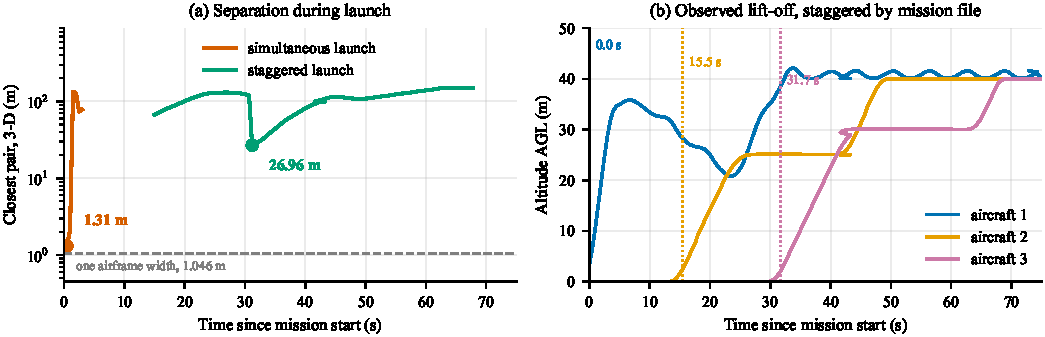
\includegraphics[width=\textwidth]{fig-launch.pdf}
\caption{Separation at launch from the recorded telemetry of three ArduCopter
autopilots. (a) Closest airborne pair in three dimensions, log scale.
Simultaneous launch brings two aircraft within 1.31\,m; staggered take-off
keeps them at least 26.96\,m apart. (b) Altitude of each aircraft, with
observed lift-off times.}
\label{fig:launch}
\end{figure*}

\textit{Sweep.} Away from the pad the aircraft never came closer than
35.16\,m. Choosing the sweep direction to finish near home brought all three
sweeps to an end 117--130\,m from the pad (Fig.~\ref{fig:sweep}). Under our
earlier rule, which ignored the end point, two aircraft finished 516\,m and
540\,m away, on the lowest battery of the flight. The path length is the same
either way.

\begin{figure}[t]
\centering
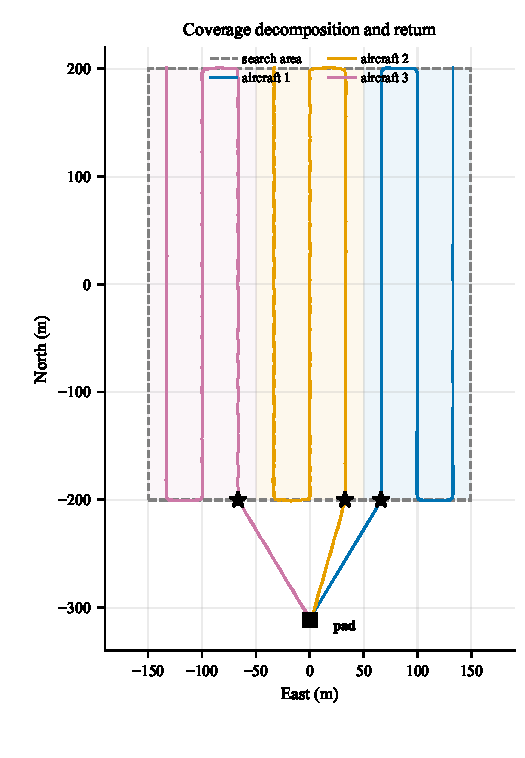
\includegraphics[width=\columnwidth]{fig-sweep.pdf}
\caption{Equal-area strips and recorded tracks. Stars mark the end of each
sweep, all within 117--130\,m of the pad.}
\label{fig:sweep}
\end{figure}

\textit{Recovery.} With the landing slots in a row the slot spacing was
1.22\,m, less than an airframe width. Placing them at the corners of the pad's
usable square raised it to 2.61\,m at no cost (Fig.~\ref{fig:pad}). The closest
airborne approach during recovery was 5.34\,m. The corner layout has one weakness:
each slot is exactly one airframe radius, 0.523\,m, from the pad edge. A
stationary aircraft on its slot fits, but any touchdown error puts part of the
airframe over the edge. Moving the slots inward would reduce the spacing that
the corners were chosen for, so the layout can only be settled once touchdown
error has been measured in flight.

\begin{figure}[t]
\centering
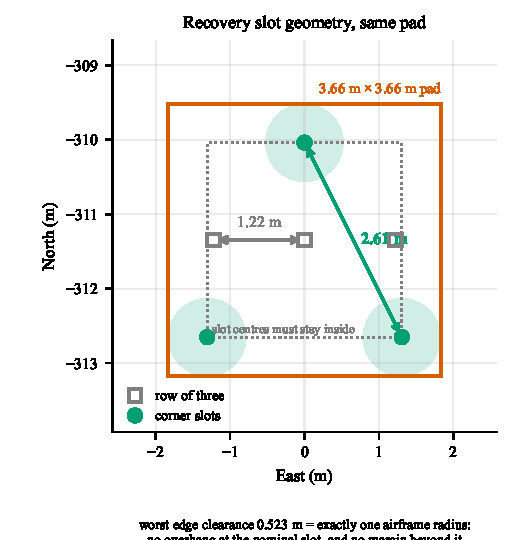
\includegraphics[width=\columnwidth]{fig-pad.pdf}
\caption{Landing slot layout on a 3.66\,m pad. Slot centres must stay half an
airframe inside the edge. A row gives 1.22\,m spacing and the corners give
2.61\,m. Discs show the 1.046\,m airframe footprint.}
\label{fig:pad}
\end{figure}

\textit{Failsafe and ground station.} In a separate run the low-battery
failsafe returned each of the three aircraft to the pad, triggering at
10\,809\,mAh consumed against a configured 10\,800\,mAh. The ground station
displayed all three aircraft at once from offline map tiles
(Fig.~\ref{fig:gcs}).

\begin{figure*}[t]
\centering
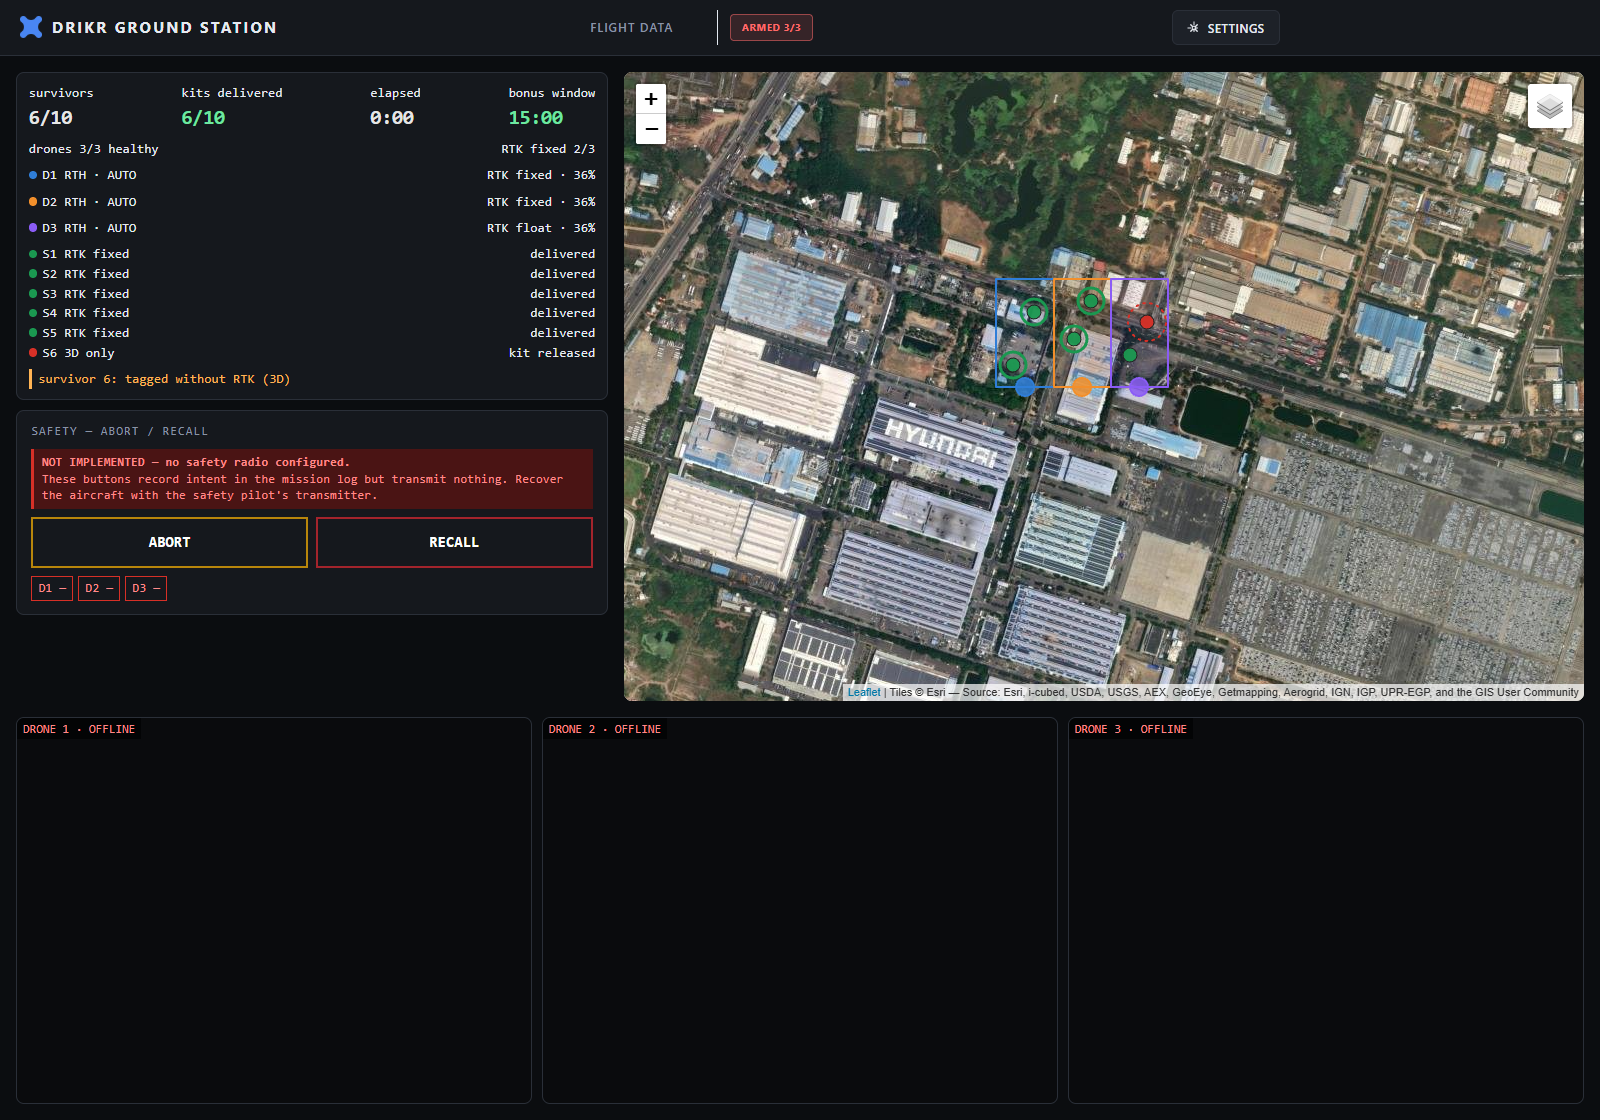
\includegraphics[width=0.94\textwidth]{gcs-dark.png}
\caption{Ground station during a simulated mission, unedited. The telemetry
comes from a test driver, not from aircraft. Six survivors have been found and
six kits dropped. Five survivors are tagged \textsc{rtk fixed} and the sixth
\textsc{3d only}; the display shows the difference because a crew sent to the
sixth must search a wider area. The safety panel states that abort and recall
are not yet transmitted. The video panels are offline because the media server
was not running.}
\label{fig:gcs}
\end{figure*}

%=============================================================================
\section{Discussion}
%=============================================================================

Several of our results say more about the design process than the aircraft.
The receiver analysis is the clearest example. We expected RTK to be the
deciding factor in coordinate accuracy, and it turned out to buy 0.16\,m of
CEP50 over SBAS, because target size and unmodelled error dominate. The link
analysis is another. The mesh was attractive for its relay capability, and the
margin calculation, not the architecture diagram, showed that it would have
been the weakest link in the system. In both cases a few lines of arithmetic
changed a decision that looked settled.

We also learned something about verification. Four times during development we
found a configuration file that was correct and reviewed but never loaded by the
running system. In one case the failsafe parameters were never applied in
simulation, so every test had run with the low-battery action switched off.
Since then we count a behaviour as shown only once the real configuration has
run end to end and its values have been read back from the running autopilot.

\subsection{Limitations}

Nothing has flown, so none of the physical effects is measured. The most
important unknown is detection recall on real flood imagery. We do not train on
images of real casualties, and our field targets will be home-made forms laid
on ground surveyed with our own RTK rover. Because the reference positions come
from the same kind of receiver as the aircraft, their errors are correlated, and
measured geolocation accuracy will look slightly better than it would against an
independent survey.

The motors publish no thrust curve, so the thrust-to-weight ratio is a
requirement until it is measured on a thrust stand. The battery model uses
typical cell parameters rather than measured ones. The accelerator throughput
figures are published values, not our own.

The system cannot see obstacles ahead. A 40\,m survey altitude clears the two-
to four-storey buildings of rural and semi-urban flood plains but not those of
Chennai or Mumbai, and flying higher is not an option because at 50\,m the target
already drops below the small-object threshold. Tall structures must be drawn
as exclusion zones, which the autopilot enforces, and an unmarked one would be
hit. The system is therefore suited to open water and low-rise flooding only.

\subsection{Data protection}

The system records the locations and images of people in distress who cannot
consent. Under India's Digital Personal Data Protection Act 2023 this is personal
data. Coordinates are kept only for the operation and deleted after handover,
images stay on the aircraft unless needed as evidence for a specific
measurement, and no image of an identifiable person is published.

%=============================================================================
\section{Conclusion and Future Work}
%=============================================================================

We have presented the design of a three-aircraft system for flood search and
relief delivery and evaluated it by analysis and simulation. Coordinate accuracy
is limited mainly by target size and unmodelled error, so any receiver better
than 2.75\,m meets a 5\,m requirement. Detecting a person in water needs 40\,m
and full-resolution tiling together. Separate single-purpose radios give every
link at least 29.7\,dB of margin, and framing overhead rather than bit rate sets
the capacity of the coordination channel. In simulation, scheduling take-off in
the mission file raised launch separation from 1.31\,m to 26.96\,m.

The next step is to build and fly the aircraft and replace the modelled figures
with measured ones, starting with thrust, pack sag, detection recall and
delivery error. Two extensions interest us beyond that. For night operation over
water, near-infrared imaging may suit better than thermal: a person in floodwater
cools towards the water's temperature, while water absorbs strongly above about
900\,nm and skin does not. And running the same tiled detection on accelerators
of decreasing capability would show how much computing a given coverage rate
really needs, which we have not found published for aerial person detection.

\section*{Acknowledgment}

We thank Dr.~Surbhi Sharma and Dr.~Mamata Gulati for their supervision and
guidance, and the Department of Electronics and Communication Engineering,
Thapar Institute of Engineering and Technology, for its support.

\begin{thebibliography}{00}
\bibitem{idmc2025grid}
Internal Displacement Monitoring Centre,
\emph{Global Report on Internal Displacement 2025}, Geneva, 2025.

\bibitem{kapoutsis2017darp}
A.~C. Kapoutsis, S.~A. Chatzichristofis, and E.~B. Kosmatopoulos,
``DARP: Divide areas algorithm for optimal multi-robot coverage path planning,''
\emph{J. Intell. Robot. Syst.}, vol.~86, pp.~663--680, 2017.

\bibitem{choset2000coverage}
H.~Choset,
``Coverage of known spaces: the boustrophedon cellular decomposition,''
\emph{Auton. Robots}, vol.~9, no.~3, pp.~247--253, 2000.

\bibitem{choi2009cbba}
H.-L. Choi, L.~Brunet, and J.~P. How,
``Consensus-based decentralized auctions for robust task allocation,''
\emph{IEEE Trans. Robot.}, vol.~25, no.~4, pp.~912--926, 2009.

\bibitem{lin2014coco}
T.-Y. Lin \emph{et al.},
``Microsoft COCO: Common objects in context,''
in \emph{Proc. ECCV}, 2014, pp.~740--755.

\bibitem{yu2020tinyperson}
X.~Yu, Y.~Gong, N.~Jiang, Q.~Ye, and Z.~Han,
``Scale match for tiny person detection,''
in \emph{Proc. IEEE/CVF WACV}, 2020.

\bibitem{akyon2022sahi}
F.~C. Akyon, S.~O. Altinuc, and A.~Temizel,
``Slicing aided hyper inference and fine-tuning for small object detection,''
in \emph{Proc. IEEE ICIP}, 2022, pp.~966--970.

\bibitem{sambolek2021sard}
S.~Sambolek and M.~Ivasic-Kos,
``Automatic person detection in search and rescue operations using deep CNN
detectors,'' \emph{IEEE Access}, vol.~9, pp.~37\,905--37\,922, 2021.

\bibitem{zhu2021visdrone}
P.~Zhu \emph{et al.},
``Detection and tracking meet drones challenge,''
\emph{IEEE Trans. Pattern Anal. Mach. Intell.}, vol.~44, no.~11,
pp.~7380--7399, 2021.

\bibitem{varga2022seadronessee}
L.~A. Varga, B.~Kiefer, M.~Messmer, and A.~Zell,
``SeaDronesSee: A maritime benchmark for detecting humans in open water,''
in \emph{Proc. IEEE/CVF WACV}, 2022.

\bibitem{mathisen2020airdrop}
S.~G. Mathisen, F.~S. Leira, H.~H. Helgesen, K.~Gryte, and T.~A. Johansen,
``Autonomous ballistic airdrop of objects from a small fixed-wing unmanned
aerial vehicle,'' \emph{Auton. Robots}, vol.~44, pp.~859--875, 2020.

\bibitem{takasu2009rtklib}
T.~Takasu and A.~Yasuda,
``Development of the low-cost RTK-GPS receiver with an open source program
package RTKLIB,'' in \emph{Proc. Int. Symp. GPS/GNSS}, 2009.

\bibitem{leishman2006helicopter}
J.~G. Leishman,
\emph{Principles of Helicopter Aerodynamics}, 2nd~ed.
Cambridge, U.K.: Cambridge Univ. Press, 2006.

\bibitem{dronerules2021}
Ministry of Civil Aviation, Government of India,
\emph{The Drone Rules, 2021}, G.S.R.~589(E), Aug.~2021.

\bibitem{ardupilot}
ArduPilot Development Team, ``ArduPilot.'' [Online]. Available:
\url{https://ardupilot.org/}

\bibitem{ubloxzedf9p}
u-blox, ``ZED-F9P high precision GNSS module,'' data sheet, 2024.

\bibitem{wfbng}
wfb-ng contributors, ``wfb-ng: long-range packet radio link based on raw
WiFi.'' [Online]. Available: \url{https://github.com/svpcom/wfb-ng}

\bibitem{elrsmavlink}
ExpressLRS Project, ``MAVLink,'' ExpressLRS documentation. [Online].
Available: \url{https://www.expresslrs.org/software/mavlink/}
\end{thebibliography}

\end{document}
